%==============================================================================
%  An Interpretable Multi-Modal Spam Detection Framework Using Explainable AI
%  and Machine Learning  --  IEEE conference format (IEEEtran)
%
%  Build:  latexmk -pdf main.tex      (or: pdflatex, bibtex, pdflatex, pdflatex)
%  Result tables in tables/ are generated by analysis/make_tables.py from
%  analysis/extended_results.json (see README.md).
%==============================================================================
\documentclass[conference]{IEEEtran}
\IEEEoverridecommandlockouts

\usepackage[T1]{fontenc}
\usepackage[utf8]{inputenc}
\usepackage{cite}
\usepackage{amsmath,amssymb,amsfonts}
\usepackage{graphicx}
\usepackage{textcomp}
\usepackage{xcolor}
\usepackage{booktabs}
\usepackage{multirow}
\usepackage{array}
\usepackage{url}
\usepackage{pgfplots}
\pgfplotsset{compat=1.17}
\usetikzlibrary{arrows.meta,positioning,calc,fit,backgrounds}

% expandable \input, so generated table bodies can be followed by \bottomrule
\makeatletter
\newcommand{\inputtable}[1]{\@@input #1 }
\makeatother
% start a new, centred row of author blocks (IEEEtran conference mode)
\makeatletter
\newcommand{\linebreakand}{%
  \end{@IEEEauthorhalign}
  \hfill\mbox{}\par
  \mbox{}\hfill\begin{@IEEEauthorhalign}
}
\makeatother
\newcommand{\tok}[1]{\texttt{\detokenize{#1}}}
\newcolumntype{L}[1]{>{\raggedright\arraybackslash}p{#1}}

\tikzset{
  blk/.style={draw=black!65, fill=gray!7, rounded corners=1.5pt, align=center,
              font=\scriptsize, minimum height=0.62cm, inner sep=2.5pt},
  mdl/.style={blk, fill=blue!7},
  xai/.style={blk, fill=orange!15},
  dat/.style={blk, fill=green!9},
  arr/.style={-{Latex[length=1.6mm]}, semithick},
}

\begin{document}
\bstctlcite{IEEEexample:BSTcontrol}

\title{An Interpretable Multi-Modal Spam Detection Framework Using Explainable AI and Machine Learning}

\author{\IEEEauthorblockN{Sonam Juneja}
\IEEEauthorblockA{\textit{Computer Science and Engineering}\\
\textit{Chandigarh University}\\
Mohali, Punjab, India\\
sonam.e11002@cumail.in}
\and
\IEEEauthorblockN{Vanshit Kumar}
\IEEEauthorblockA{\textit{Computer Science and Engineering}\\
\textit{Chandigarh University}\\
Mohali, Punjab, India\\
23bcs10087@cuchd.in}
\and
\IEEEauthorblockN{Aariz Amaan}
\IEEEauthorblockA{\textit{Computer Science and Engineering}\\
\textit{Chandigarh University}\\
Mohali, Punjab, India\\
23bcs10422@cuchd.in}
\linebreakand
\IEEEauthorblockN{Naman}
\IEEEauthorblockA{\textit{Computer Science and Engineering}\\
\textit{Chandigarh University}\\
Mohali, Punjab, India\\
23bcs11036@cuchd.in}
\and
\IEEEauthorblockN{Aditi Arya}
\IEEEauthorblockA{\textit{Computer Science and Engineering}\\
\textit{Chandigarh University}\\
Mohali, Punjab, India\\
23bcs11535@cuchd.in}
\and
\IEEEauthorblockN{Avish Kumar Dubey}
\IEEEauthorblockA{\textit{Computer Science and Engineering}\\
\textit{Chandigarh University}\\
Mohali, Punjab, India\\
23bcs13898@cuchd.in}}

\maketitle

\begin{abstract}
Scam messages reach users through several channels, yet the machine-learning
filters that intercept them usually return a verdict without a reason, leaving
errors and dataset artefacts invisible. This paper presents an interpretable
multi-modal framework that detects fraudulent SMS and e-mail messages and
explains every decision. Each channel is served by a specialist pipeline that
maps URLs, phone numbers, currency amounts and numbers to readable placeholder
tokens, combines uni-/bi-gram TF--IDF features with fifteen stylometric
statistics, and fuses Logistic Regression, Random Forest and XGBoost by soft
voting weighted with cross-validated F1. LIME explains the full ensemble
locally, while exact TreeSHAP attributes the boosted-tree component locally
and globally. On held-out splits of the UCI SMS Spam Collection (5,158
messages) and the Enron-Spam corpus (12,000 messages), the ensemble reaches
98.55\% accuracy (ROC-AUC 0.9941) on SMS and 98.25\% (ROC-AUC 0.9983) on
e-mail. Paired McNemar and DeLong tests show that it significantly outperforms
both tree learners on e-mail ($p \le 0.003$, Holm-corrected) and is
statistically indistinguishable from Logistic Regression. Deleting the five
words ranked highest by LIME lowers the spam probability 5.6--20 times more
than deleting random words, supporting explanation faithfulness. Global
attributions show that stylometric features dominate SMS decisions and expose
a corpus shortcut: the token \tok{enron} occurs in 42\% of legitimate test
e-mails and in no spam, and appending it to spam e-mails flips 35.5\% of the
ensemble's detections (91.7\% for XGBoost alone). We further show that channel
specialisation is essential---cross-channel transfer is near chance---and
quantify the cost of heuristic routing.
\end{abstract}

\begin{IEEEkeywords}
Spam detection, smishing, phishing, explainable artificial intelligence, SHAP,
LIME, ensemble learning, shortcut learning, stylometry.
\end{IEEEkeywords}

%==============================================================================
\section{Introduction}
%==============================================================================

Fraudulent messaging remains the most frequently reported form of cybercrime.
In 2025 the FBI's Internet Crime Complaint Center received more than one
million complaints with reported losses of US\$20.9 billion; phishing and
spoofing was again the most reported category (191,561 complaints), and
22,364 complaints involved artificial intelligence (AI)~\cite{fbi2026ic3}. The
threat is changing in character as well as volume. Large language models
(LLMs) can generate persuasive, personalised phishing at negligible
cost~\cite{heiding2024devising,yao2024survey,xu2025llm4sec}, and scams have
followed banking and one-time-password traffic onto SMS
(``smishing'')~\cite{mehmood2024smishing,schwarz2025smishing}.

Machine-learning filters have been the standard defence since the first
probabilistic spam filters~\cite{sahami1998bayesian,drucker1999svm}, and
modern deep and transformer models report excellent benchmark
accuracy~\cite{zavrak2023email,jamal2024improved,roumeliotis2024next}. Most
deployed filters, however, are black boxes: a message is blocked and neither
the user, the analyst nor an auditor can say why. Aggregate accuracy can
conceal systematic errors and shortcuts---spurious cues that happen to
separate the classes in a particular dataset~\cite{geirhos2020shortcut,du2024shortcut}.
At the same time, data-protection and AI legislation has raised expectations
of transparency and accountability for automated processing of personal
data~\cite{eu2016gdpr,eu2024aiact,india2023dpdp}, and explainable AI (XAI) has
matured into a broad toolkit~\cite{ali2023xai,longo2024xai,rjoub2023survey}.

Three gaps motivate this work. First, most detectors target a single channel,
although SMS and e-mail scams are two faces of one problem with very
different statistics (a median of 12 versus 155 words and 12\% versus 48\%
spam in the corpora used here). Second, explanations are usually shown as
illustrations of individual predictions rather than evaluated for
faithfulness~\cite{nauta2023anecdotal,lyu2024faithful} or used to audit what
the model has learned. Third, model comparisons on near-saturated benchmarks
are rarely accompanied by uncertainty estimates, so differences in the third
decimal place are hard to interpret~\cite{dietterich1998approximate}.

We address these gaps with an interpretable, multi-modal spam detection
framework. Throughout the paper, \emph{modality} denotes the messaging channel
(SMS or e-mail); both are text, so the framework is multi-channel rather than
multimodal in the sense of combining text with images or audio. Our
contributions are:
\begin{enumerate}
  \item An interpretability-first pipeline with one specialist per channel:
        high-signal entities become readable placeholder tokens, TF--IDF
        features are combined with fifteen named stylometric statistics, and
        Logistic Regression (LR), Random Forest (RF) and XGBoost (XGB) are fused
        by performance-weighted soft voting. Training takes about 14\,s (SMS)
        and 77\,s (e-mail) on a commodity CPU.
  \item A statistically grounded evaluation: bootstrap confidence intervals,
        exact McNemar and DeLong tests with Holm correction, Matthews
        correlation coefficient (MCC) and PR-AUC, together with an
        end-to-end evaluation of the channel router and of cross-channel
        transfer.
  \item A dual explanation layer---LIME over the full ensemble and exact
        TreeSHAP over the boosted component---whose local faithfulness is
        tested with a word-deletion experiment.
  \item An explanation-driven audit that discovers a corpus shortcut
        (\tok{enron}), quantifies how far it can be exploited by a one-word
        insertion, and identifies a subtle sparse-versus-dense pitfall that
        silently invalidates SHAP explanations of XGBoost text models.
\end{enumerate}

Section~\ref{sec:related} reviews related work, Section~\ref{sec:method}
describes the framework, Section~\ref{sec:setup} the experimental protocol,
Section~\ref{sec:results} the results, Section~\ref{sec:discussion} discusses
implications and limitations, and Section~\ref{sec:conclusion} concludes.

%==============================================================================
\section{Related Work}\label{sec:related}
%==============================================================================

\subsection{SMS Spam and Smishing Detection}

Reproducible SMS research began with the UCI SMS Spam
Collection~\cite{almeida2011sms}. Recent detectors are predominantly deep or
transformer based: Ghourabi and Alohaly combined pre-trained transformer
embeddings with ensemble learning~\cite{ghourabi2023enhancing}; Mehmood
\emph{et al.} designed a deep smishing detector aimed at reducing false
positives~\cite{mehmood2024smishing}; Al-Kabbi \emph{et al.} proposed a
two-level feature-fusion filter against fraudulent writing
styles~\cite{alkabbi2024hierarchical}; and Nguyen-Xuan and Nguyen introduced
a compound-aware encoder-only transformer~\cite{nguyenxuan2026compound}.
Schwarz \emph{et al.} studied smishing from the messaging-platform side,
classifying application-to-person traffic by
industry~\cite{schwarz2025smishing}. Hur \emph{et al.} examined whether LLMs
improve on machine-learning, deep-learning and encoder models for SMS
spam~\cite{hur2026llm}, while \c{S}ahin \emph{et al.} benchmarked classical
learners across text representations under imbalanced short-text conditions,
emphasising precision and specificity because blocking legitimate messages is
costly~\cite{sahin2026revisiting}.

Coverage of other languages is growing, including Swahili~\cite{mambina2024swahili},
Dravidian languages with hand-crafted meta-data
features~\cite{ramanujam2025dravidian}, and cross-lingual detection with
GAN-based augmentation for imbalanced data~\cite{filali2026crosslingual}.
Robustness is an open concern: Salman \emph{et al.} released a new SMS
dataset and analysed spammers' evasive techniques against several
models~\cite{salman2024evasive}, and later evaluated commercial apps,
third-party services and open-weight models under perceptible and
imperceptible attacks~\cite{salman2026johnny}. Rassam and Shaddad studied the
robustness and interpretability of naive Bayes and a compact CNN under
adversarial attack~\cite{rassam2026robustness}, and SpamDam pursues
privacy-preserving, adversary-resistant SMS filtering~\cite{li2024spamdam}.

\subsection{E-mail Spam and Phishing Detection}

E-mail filtering moved from naive Bayes~\cite{sahami1998bayesian,metsis2006spam}
and support vector machines~\cite{drucker1999svm} to deep architectures such
as hierarchical attention networks~\cite{zavrak2023email}, hybrid networks
with adaptive optimisation~\cite{hosseinzadeh2025phishing}, vector-similarity
search over transformer embeddings~\cite{patra2025vector} and graph attention
over content and metadata~\cite{safran2025phishinggnn}; a systematic review
covers deep phishing-e-mail detectors~\cite{thakur2023systematic}. Transformers
and LLMs now dominate recent work: fine-tuned models for three-way
phishing/spam/ham classification~\cite{jamal2024improved}, comparative
fine-tuning of LLMs, NLP models and CNNs~\cite{roumeliotis2024next},
few-shot benchmarks against naive Bayes and LightGBM
baselines~\cite{labonne2023spamt5}, DistilBERT embeddings with neural
classifiers~\cite{reddy2025llm}, comparisons of ML and LLMs with embedded URL
analysis~\cite{tarapiah2025llm}, and multilingual LLMs for low-resource Kazakh
spam~\cite{mukhammedali2026kazakh}. Mel\'{e}ndez \emph{et al.} contrasted
traditional models with transformers for phishing
e-mail~\cite{melendez2024comparative}. Ensembles remain competitive through
stacking~\cite{tian2025stacking}, decision fusion~\cite{zhang2024ensemble} and
interpretable meta-learners~\cite{kshirsagar2025metalearner}. Few studies
cover both channels: Maqsood \emph{et al.} proposed a deep framework for SMS
and e-mail~\cite{maqsood2023intelligent}, and Hadi \emph{et al.} fused
shallow lexical features (bag-of-words, TF--IDF, lexical statistics) with
deep contextual features~\cite{hadi2026hybrid}.

The adversary is also changing. LLMs can author effective phishing at
scale~\cite{heiding2024devising}; Opara \emph{et al.} evaluated how spam
filters handle AI-generated phishing and proposed stylometric
detection~\cite{opara2025evaluating}; detectors must generalise across
generator models~\cite{gutierrez2026crossmodel,ghawa2026hybrid}; persuasion
principles in phishing have been quantified with LLMs~\cite{pan2026psychology};
and spear phishing has been surveyed comprehensively~\cite{birthriya2025spear}.

\subsection{Explainable AI for Message Filtering}

Surveys chart the XAI landscape~\cite{ali2023xai,schwalbe2024taxonomy,bodria2023benchmarking,saarela2024recent,longo2024xai}
and its use in cybersecurity~\cite{rjoub2023survey,reynaud2025review}. LIME
fits a sparse local surrogate around one prediction~\cite{ribeiro2016lime};
SHAP assigns additive Shapley-value attributions~\cite{lundberg2017shap} and
admits an exact polynomial-time algorithm for tree
ensembles~\cite{lundberg2020treeshap}. Both are among the most widely used
post-hoc tools~\cite{vimbi2024interpreting,saarela2024recent}. In message
filtering, explanations have accompanied transformer SMS
detectors~\cite{uddin2025explainabledetector}, smishing
detectors~\cite{prince2026explainable} and transformer phishing
models~\cite{uddin2026explainable}; SHAP has guided feature selection for spam
detection~\cite{shambour2025quantum}; SHAP and LIME have been compared on
boosting models for phishing URLs~\cite{panthi2026shaplime}; ChatSpamDetector
uses an LLM to produce human-readable rationales~\cite{koide2026chatspamdetector};
and fuzzy rule bases offer intrinsic interpretability~\cite{jasim2026fuzzy}.

Explanations are not trustworthy by default. Faithfulness---whether an
explanation reflects the model's actual reasoning---must be
measured~\cite{nauta2023anecdotal,lyu2024faithful,deyoung2020eraser};
attention weights are an unreliable proxy~\cite{jain2019attention,lyu2024faithful,zhao2024explainability};
explainers frequently disagree~\cite{krishna2024disagreement,mitrut2024clarity};
explanations can be manipulated~\cite{baniecki2024adversarial}; and
human-centred studies~\cite{kim2024human} warn that users may over-trust AI
advice~\cite{romeo2025automation}.

\subsection{Shortcut Learning and Dataset Bias}

Models may exploit spurious cues that correlate with labels in the training
data rather than the intended concept, the ``Clever Hans''
effect~\cite{geirhos2020shortcut,pathak2026cleverhans}. In NLP such shortcuts
originate in dataset biases~\cite{dogra2024shortcut} and persist in
LLMs~\cite{du2024shortcut}. Spam corpora are vulnerable because legitimate
messages are often drawn from a single organisation, so organisation names
and internal jargon can become label proxies. Explanations are a natural
instrument for exposing such shortcuts~\cite{dogra2024shortcut}.

\subsection{Positioning}

Table~\ref{tab:related} contrasts representative recent studies. Most address
a single channel, and explanations, where present, mainly illustrate
individual predictions. We combine two channel specialists with a dual
explanation layer, test the faithfulness of the local explanations, use the
global explanations to audit the model, and compare learners with paired
significance tests.

\begin{table*}[!t]
\caption{Representative Recent Studies Compared With This Work}
\label{tab:related}
\centering
\footnotesize
\begin{tabular}{@{}L{3.1cm}cL{2.0cm}L{5.0cm}L{5.3cm}@{}}
\toprule
\textbf{Study} & \textbf{Year} & \textbf{Channel} & \textbf{Approach} & \textbf{Explanation} \\
\midrule
Ghourabi \& Alohaly~\cite{ghourabi2023enhancing} & 2023 & SMS & Transformer embeddings + ensemble & -- \\
Maqsood \emph{et al.}~\cite{maqsood2023intelligent} & 2023 & SMS + e-mail & Deep learning framework & -- \\
Salman \emph{et al.}~\cite{salman2024evasive} & 2024 & SMS & ML/DL models under evasive techniques; new dataset & -- \\
Roumeliotis \emph{et al.}~\cite{roumeliotis2024next} & 2024 & E-mail & Fine-tuned LLMs, NLP models and CNNs & -- \\
Mel\'{e}ndez \emph{et al.}~\cite{melendez2024comparative} & 2024 & E-mail (phishing) & Traditional ML vs.\ transformers & -- \\
Uddin \emph{et al.}~\cite{uddin2025explainabledetector} & 2025 & SMS & Transformer language model & Post-hoc explainability analysis \\
Kshirsagar \emph{et al.}~\cite{kshirsagar2025metalearner} & 2025 & E-mail & Meta-learner ensembles & Interpretable by design \\
Uddin \emph{et al.}~\cite{uddin2026explainable} & 2026 & E-mail (phishing) & Fine-tuned transformer & Post-hoc explanations \\
Koide \emph{et al.}~\cite{koide2026chatspamdetector} & 2026 & E-mail (phishing) & LLM-based detection & LLM-generated rationale \\
Jasim \emph{et al.}~\cite{jasim2026fuzzy} & 2026 & SMS & Fuzzy logic + BiLSTM & Fuzzy rules \\
Prince \emph{et al.}~\cite{prince2026explainable} & 2026 & SMS (smishing) & Hybrid transformer feature fusion & Post-hoc XAI \\
Hadi \emph{et al.}~\cite{hadi2026hybrid} & 2026 & SMS + e-mail & Shallow lexical + deep contextual features & -- \\
\midrule
\textbf{This work} & 2026 & SMS + e-mail (routed specialists) & TF--IDF + stylometry; LR, RF, XGB fused by F1-weighted soft voting & LIME (full ensemble) + exact TreeSHAP; deletion faithfulness test; shortcut audit \\
\bottomrule
\end{tabular}
\end{table*}

%==============================================================================
\section{Proposed Framework}\label{sec:method}
%==============================================================================

Fig.~\ref{fig:arch} shows the architecture. A message $x$ is routed to the
specialist of its channel $c \in \{\textsc{sms}, \textsc{email}\}$; each
specialist has its own normalisation, feature space and trained ensemble, and
returns a label $\hat{y}\in\{\text{ham},\text{spam}\}$, a spam probability and
explanations.

\begin{figure*}[!t]
\centering
\resizebox{\textwidth}{!}{%
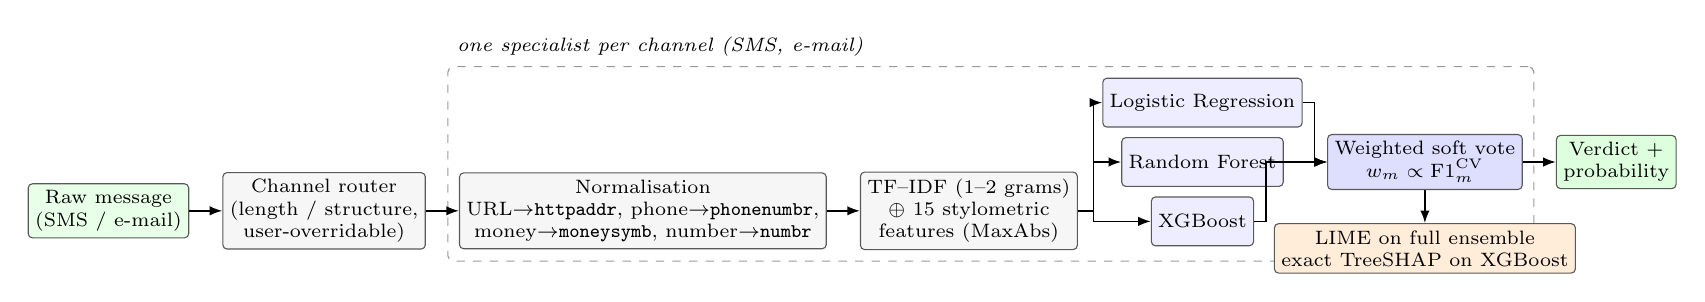
\begin{tikzpicture}[node distance=0.32cm and 0.42cm]
  \node[dat] (msg) {Raw message\\(SMS / e-mail)};
  \node[blk, right=of msg] (rt) {Channel router\\(length / structure,\\user-overridable)};
  \node[blk, right=of rt, minimum width=3.0cm] (norm) {Normalisation\\URL$\to$\tok{httpaddr}, phone$\to$\tok{phonenumbr},\\money$\to$\tok{moneysymb}, number$\to$\tok{numbr}};
  \node[blk, right=of norm, minimum width=2.5cm] (feat) {TF--IDF (1--2 grams)\\$\oplus$ 15 stylometric\\features (MaxAbs)};
  \node[mdl, right=0.55cm of feat, yshift=0.62cm] (rf) {Random Forest};
  \node[mdl, above=0.12cm of rf] (lr) {Logistic Regression};
  \node[mdl, below=0.12cm of rf] (xgb) {XGBoost};
  \node[mdl, right=0.55cm of rf, fill=blue!13] (ens) {Weighted soft vote\\$w_m \propto \mathrm{F1}^{\mathrm{CV}}_m$};
  \node[dat, right=0.42cm of ens, fill=green!13] (out) {Verdict +\\probability};
  \node[xai, below=0.42cm of ens, minimum width=3.6cm] (xai) {LIME on full ensemble\\exact TreeSHAP on XGBoost};
  \begin{scope}[on background layer]
    \node[draw=black!40, dashed, rounded corners=2pt, fit=(norm)(feat)(lr)(xgb)(ens), inner sep=4pt,
          label={[font=\scriptsize\itshape, anchor=south west]north west:one specialist per channel (SMS, e-mail)}] {};
  \end{scope}
  \draw[arr] (msg) -- (rt);
  \draw[arr] (rt) -- (norm);
  \draw[arr] (norm) -- (feat);
  \draw[arr] (feat.east) -- ++(0.2,0) |- (lr.west);
  \draw[arr] (feat.east) -- ++(0.2,0) |- (rf.west);
  \draw[arr] (feat.east) -- ++(0.2,0) |- (xgb.west);
  \draw[arr] (lr.east) -- ++(0.15,0) |- (ens.west);
  \draw[arr] (rf.east) -- (ens.west);
  \draw[arr] (xgb.east) -- ++(0.15,0) |- (ens.west);
  \draw[arr] (ens) -- (out);
  \draw[arr] (ens) -- (xai);
\end{tikzpicture}}
\caption{Architecture of the proposed framework. Each channel has its own
normalisation, feature space and ensemble; the explanation layer returns a
local explanation with every verdict and global summaries of each model.}
\label{fig:arch}
\end{figure*}

\subsection{Interpretability-Preserving Normalisation}

Text is lower-cased, HTML tags are stripped, and high-signal entities are
\emph{mapped} rather than deleted: URLs become \tok{httpaddr}, e-mail addresses
\tok{emailaddr}, currency amounts \tok{moneysymb}, phone numbers
\tok{phonenumbr} and remaining numbers \tok{numbr}; other non-letters are
removed. Deleting these entities would discard some of the strongest scam
signals, whereas readable placeholders can appear verbatim in an explanation.
No stemming or lemmatisation is applied, so every token in an explanation is
a surface word form a non-expert can recognise.

\subsection{Feature Representation}

The normalised text is vectorised with sublinear TF--IDF over uni- and
bi-grams~\cite{salton1988term}. For term $t$ in document $d$ of a training
corpus with $N$ documents,
\begin{equation}
  w_{t,d} = \bigl(1+\ln \mathrm{tf}_{t,d}\bigr)\left(\ln\frac{1+N}{1+\mathrm{df}_t}+1\right),
  \label{eq:tfidf}
\end{equation}
after which each document vector is $\ell_2$-normalised. Vocabularies are
capped at 3,000 terms (SMS, $\mathrm{df}\ge 2$) and 5,000 terms (e-mail,
$\mathrm{df}\ge 3$). Fifteen stylometric statistics are computed on the
\emph{raw} message (Table~\ref{tab:features}); they are scaled by their
training-set maximum absolute value and appended, giving 3,015 (SMS) and 5,015
(e-mail) dimensions. Their names are written in upper case so that they are
visually distinct from vocabulary in every explanation.

\begin{table}[!t]
\caption{Engineered Stylometric Features (Computed on the Raw Message)}
\label{tab:features}
\centering
\footnotesize
\begin{tabular}{@{}L{3.05cm}L{4.7cm}@{}}
\toprule
\textbf{Feature} & \textbf{Description} \\
\midrule
\tok{CHAR_COUNT}, \tok{WORD_COUNT} & Length in characters / words \\
\tok{AVG_WORD_LEN} & Mean word length \\
\tok{DIGIT_RATIO} & Share of characters that are digits \\
\tok{UPPERCASE_RATIO} & Share of letters in upper case \\
\tok{ALLCAPS_WORDS} & Words written fully in capitals \\
\tok{PUNCT_RATIO} & Share of punctuation characters \\
\tok{SPECIAL_CHAR_RATIO} & Share of non-alphanumeric characters \\
\tok{NUM_EXCLAMATIONS} & Count of ``!'' \\
\tok{NUM_QUESTIONS} & Count of ``?'' \\
\tok{NUM_CURRENCY} & Currency symbols and money amounts \\
\tok{NUM_URLS}, \tok{NUM_EMAILS} & Detected links / e-mail addresses \\
\tok{NUM_PHONES} & Detected phone numbers \\
\tok{SPAM_KEYWORDS} & Hits in a 46-word, human-auditable scam lexicon \\
\bottomrule
\end{tabular}
\end{table}

\subsection{Heterogeneous Base Learners}

Three learners with different inductive biases provide ensemble
diversity~\cite{mohammed2023ensemble}: a linear model, a bagged tree ensemble
and a boosted tree ensemble. LR (liblinear, $C=1$) and RF~\cite{breiman2001random}
(250 trees, minimum leaf size 2) use balanced class weights; XGBoost~\cite{chen2016xgboost}
(300 trees, depth 6, learning rate 0.1, row/column subsampling 0.9/0.8,
histogram method) uses $\mathrm{scale\_pos\_weight}=N_{\text{ham}}/N_{\text{spam}}$
on the training split. Class re-weighting was preferred to synthetic
oversampling so that every training example remains a real, explainable
message. All models use scikit-learn~\cite{pedregosa2011scikit} or the XGBoost
library with a fixed seed (42).

\subsection{Performance-Weighted Soft Voting}

Let $p_m(\text{spam}\mid x)$ be the probability returned by learner $m$ and
$\mathrm{F1}^{\mathrm{CV}}_m$ its mean F1 in stratified 5-fold
cross-validation on the training split. The ensemble computes
\begin{align}
  p(\text{spam}\mid x) &= \sum_{m=1}^{3} w_m\,p_m(\text{spam}\mid x), \label{eq:ensemble}\\
  w_m &= \frac{\mathrm{F1}^{\mathrm{CV}}_m}{\sum_{k=1}^{3}\mathrm{F1}^{\mathrm{CV}}_k}, \label{eq:weights}
\end{align}
and predicts spam when $p(\text{spam}\mid x)\ge 0.5$. The resulting weights are
0.3329/0.3331/0.3340 (LR/RF/XGB) for SMS and 0.3356/0.3311/0.3333 for e-mail:
the learners are comparably strong, so any benefit of the ensemble stems from
their diversity rather than from a dominant member.

\subsection{Channel Router}

At inference time a transparent rule selects the specialist: a message is
treated as e-mail if it is longer than 280 characters, contains a line break,
or contains one of the cue words \emph{subject}, \emph{dear},
\emph{regards}, \emph{sincerely}, \emph{unsubscribe} or \emph{attached};
otherwise it is treated as SMS. The user can override the choice in the
application. Section~\ref{sec:routing} measures the cost of this heuristic.

\subsection{Explanation Layer}

\emph{Local, model-agnostic (LIME).} LIME~\cite{ribeiro2016lime} perturbs the
raw message by removing words, re-scores 1,000 perturbations through the
\emph{entire} pipeline (normalisation, features and ensemble) and fits a
locally weighted linear surrogate
\begin{equation}
  \xi(x)=\arg\min_{g\in\mathcal{G}}\;\mathcal{L}(f,g,\pi_x)+\Omega(g),
\end{equation}
where $f$ is the ensemble, $\pi_x$ a proximity kernel and $\Omega$ limits the
explanation to the ten most influential words. Because LIME queries the
deployed pipeline, it explains the complete ensemble.

\emph{Exact attributions (TreeSHAP).} For the XGBoost component, SHAP values
$\phi_j$ decompose the log-odds output additively,
$f_{\text{XGB}}(x)=\phi_0+\sum_{j}\phi_j(x)$~\cite{lundberg2017shap}, and are
computed exactly in polynomial time by TreeSHAP~\cite{lundberg2020treeshap}.
Global importance is the mean absolute attribution over a set $S$ of 800
held-out messages, $I_j=\frac{1}{|S|}\sum_{x\in S}|\phi_j(x)|$.

\emph{Implementation pitfall.} XGBoost treats entries that are \emph{not
stored} in a sparse matrix as missing values, whereas a dense array turns
them into genuine zeros that follow a different branch. Explaining a model
trained on sparse TF--IDF matrices with a densified copy of the input
therefore explains a different function: in our pipeline, densification
changes the XGBoost verdict for 729 of 1,032 SMS and 1,182 of 2,400 e-mail
test messages. All attributions in this paper are computed with XGBoost's
native TreeSHAP on exactly the sparse matrix the model scores, so that they
sum to the deployed model's output.

%==============================================================================
\section{Experimental Setup}\label{sec:setup}
%==============================================================================

\subsection{Datasets}

Table~\ref{tab:data} summarises the corpora after removing empty and duplicate
messages. The UCI SMS Spam Collection~\cite{almeida2011sms} is used in full.
For e-mail we use the Enron-Spam corpus~\cite{metsis2006spam} (subject and
body, truncated to 8,000 characters), drawing a class-stratified sample of
12,000 messages from the de-duplicated corpus to keep the full pipeline
laptop-friendly. The channels differ sharply in length and class balance,
which motivates channel-specific models.

\begin{table}[!t]
\caption{Corpora After Cleaning and De-duplication}
\label{tab:data}
\centering
\footnotesize
\setlength{\tabcolsep}{4pt}
\begin{tabular}{@{}lrrrrr@{}}
\toprule
\textbf{Channel} & \textbf{Messages} & \textbf{Spam} & \textbf{Median words} & \textbf{Train} & \textbf{Test} \\
\midrule
SMS~\cite{almeida2011sms} & 5,158 & 642 (12.4\%) & 12 & 4,126 & 1,032 \\
E-mail~\cite{metsis2006spam} & 12,000 & 5,792 (48.3\%) & 155 & 9,600 & 2,400 \\
\bottomrule
\end{tabular}
\end{table}

\subsection{Protocol and Metrics}

Each corpus is split 80/20 with stratification (seed 42). Vectorisers,
scalers, cross-validation weights and models are fitted on the training split
only, and the test split is used once for final evaluation. We report
accuracy, precision, recall, F1, MCC (preferred for imbalanced binary
problems~\cite{chicco2020mcc}), ROC-AUC, PR-AUC and the Brier score of the
predicted probabilities.

\subsection{Statistical Analysis}

Uncertainty is quantified with 95\% percentile bootstrap confidence intervals
over 2,000 resamples of the test set~\cite{efron1993bootstrap}. The ensemble is
compared with each base learner on the \emph{same} test messages using the
exact McNemar test on discordant predictions~\cite{mcnemar1947note,dietterich1998approximate}
and DeLong's test for correlated ROC curves~\cite{delong1988comparing}; $p$-values
are Holm-corrected within each channel~\cite{holm1979simple}.

\subsection{Additional Analyses}

\emph{Routing and transfer.} The router is evaluated on the pooled test sets
(3,432 messages) against oracle routing, and each specialist is applied to the
other channel's test set.
\emph{Explanation faithfulness.} Following the comprehensiveness idea of
ERASER~\cite{deyoung2020eraser}, for correctly detected spam messages we
remove all occurrences of the top-$k$ words ranked by LIME ($k\in\{1,3,5\}$)
and record the drop in ensemble spam probability, compared with removing $k$
random words (10 draws). We use 60 SMS and 25 e-mail messages because each
explanation requires 1,000 pipeline evaluations.
\emph{Shortcut probe.} For the token surfaced by the global attributions we
measure (i) deletion of the token from legitimate test e-mails and (ii)
insertion of a single occurrence into spam test e-mails.

\subsection{Implementation}

The framework is implemented in Python~3.12 with scikit-learn, XGBoost, SHAP
and LIME, and served through a four-tab Streamlit application (detector,
model performance, global explanations, documentation). A 13-check automated
smoke test covers data loading, both detectors, LIME, SHAP and a simulated
application session. All timings were measured on a 10-core ARM64 CPU without
a GPU; re-running the training code reproduces the reported metrics exactly.

%==============================================================================
\section{Results}\label{sec:results}
%==============================================================================

\begin{table*}[!t]
\caption{Held-Out Test Performance With 95\% Bootstrap Confidence Intervals (SMS: $n=1{,}032$; E-mail: $n=2{,}400$). Lower Brier Is Better.}
\label{tab:results}
\centering
\footnotesize
\setlength{\tabcolsep}{4.2pt}
\begin{tabular}{@{}llcccccccc@{}}
\toprule
\textbf{Channel} & \textbf{Model} & \textbf{Accuracy} & \textbf{Precision} & \textbf{Recall} & \textbf{F1} & \textbf{MCC} & \textbf{ROC-AUC} & \textbf{PR-AUC} & \textbf{Brier} \\
\midrule
\inputtable{tables/results.tex}
\bottomrule
\end{tabular}
\end{table*}

\subsection{Classification Performance}

Table~\ref{tab:results} reports all four systems on both channels and
Fig.~\ref{fig:roc} shows the ROC curves. The ensemble reaches 98.55\% accuracy
on SMS and 98.25\% on e-mail. On SMS it attains the highest precision
(0.9669), the lowest false-positive rate (4 of 904 legitimate messages, tied
with XGBoost), the best PR-AUC (0.9790) and the best Brier score (0.0130), and
its ROC-AUC (0.9941) ties the best base learners to four decimals. On e-mail it
has the highest recall (0.9940; 7 of 1,158 spam messages missed) and the
highest ROC-AUC (0.9983) and PR-AUC (0.9980). LR, however, is a remarkably
strong baseline: it matches the ensemble's SMS accuracy and slightly exceeds
it in SMS F1 and in e-mail accuracy and F1. The confidence intervals of all
systems overlap substantially on SMS, where the test set contains only 128
spam messages.

The two specialists err in opposite directions: the SMS ensemble favours
precision (4 false positives, 11 false negatives), the e-mail ensemble favours
recall (35 false positives, 7 false negatives). On SMS, false alarms are
costly because a suppressed message may be a one-time password, so this
profile suits the channel.

\begin{figure*}[!t]
\centering
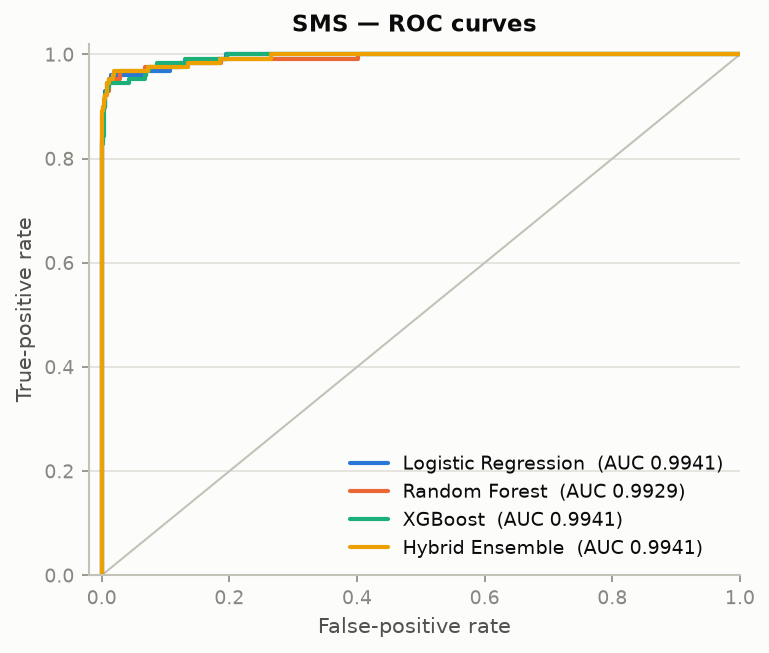
\includegraphics[width=0.40\textwidth]{figures/roc_sms.png}\hspace{0.05\textwidth}%
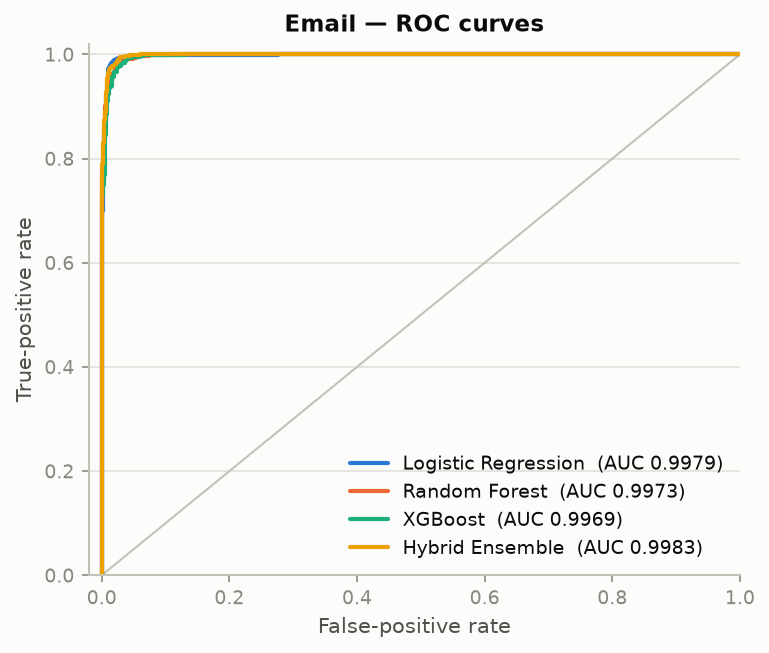
\includegraphics[width=0.40\textwidth]{figures/roc_email.png}
\caption{ROC curves of the four systems on the held-out SMS (left) and e-mail
(right) test sets. All systems exceed 0.99 AUC; differences are resolved by
the paired tests in Table~\ref{tab:significance}.}
\label{fig:roc}
\end{figure*}

\subsection{Statistical Significance}

Table~\ref{tab:significance} lists the paired tests. On SMS no difference is
significant: the ensemble and each base learner disagree on at most eight
messages. On e-mail the ensemble is significantly better than both tree
models on discordant predictions (McNemar: 24 vs.\ 5 messages against RF and
22 vs.\ 4 against XGB; Holm-corrected $p=0.002$) and in ROC-AUC (DeLong,
Holm-corrected $p\le0.003$), but it is statistically indistinguishable from
LR (11 vs.\ 13 discordant messages, $p=0.84$). Combining a linear model with
tree ensembles therefore lifts the tree models to LR's level and improves the
ranking metrics, but on these corpora it does not surpass a well-regularised
linear model on TF--IDF features.

\begin{table}[!t]
\caption{Paired Tests: Ensemble vs.\ Base Learners. $b/c$: Messages Only the Ensemble / Only the Base Learner Classifies Correctly. $p$-Values Holm-Corrected.}
\label{tab:significance}
\centering
\footnotesize
\setlength{\tabcolsep}{3.5pt}
\begin{tabular}{@{}llccccc@{}}
\toprule
 & & \multicolumn{2}{c}{\textbf{McNemar}} & \multicolumn{3}{c}{\textbf{DeLong (ROC-AUC)}} \\
\cmidrule(lr){3-4}\cmidrule(l){5-7}
\textbf{Ch.} & \textbf{Comparison} & $b/c$ & $p$ & $\Delta$AUC & $z$ & $p$ \\
\midrule
\inputtable{tables/significance.tex}
\bottomrule
\end{tabular}
\end{table}

\subsection{Routing and Cross-Channel Transfer}\label{sec:routing}

The specialists do not transfer (Table~\ref{tab:routing}). Applied to e-mail,
the SMS model is at chance level (ROC-AUC 0.53, MCC 0.04); applied to SMS, the
e-mail model labels 88\% of legitimate messages as spam. Channel-specific
training is therefore essential. The router assigns 96.4\% of SMS and 85.1\% of
e-mail test messages to the correct specialist; misrouted e-mails are short
messages without cue words, and the SMS specialist classifies only 42.3\% of
them correctly. Consequently, end-to-end accuracy on the pooled test sets
drops from 98.34\% with oracle routing to 92.16\% with automatic routing. The
classifiers are accurate; the heuristic router is the weakest component of
the deployed system, which is why the application exposes a manual override.

\begin{table}[!t]
\caption{Routing and Cross-Channel Transfer of the Ensembles (Pooled Test Set: 3,432 Messages)}
\label{tab:routing}
\centering
\footnotesize
\setlength{\tabcolsep}{3.2pt}
\begin{tabular}{@{}lccccc@{}}
\toprule
\textbf{Setting} & \textbf{Acc.} & \textbf{F1} & \textbf{MCC} & \textbf{AUC} & \textbf{FPR} \\
\midrule
\inputtable{tables/routing.tex}
\bottomrule
\end{tabular}
\end{table}

\subsection{Local Explanations}

Fig.~\ref{fig:local} explains an illustrative smishing message composed by the
authors and absent from both corpora: ``URGENT! You have WON a \pounds 2,000
cash prize GUARANTEED. Call 09061701461 now or visit www.claim-your-prize.com
to claim!'' All three learners vote spam (LR 1.000, RF 0.987, XGB 1.000;
ensemble 0.996). LIME ranks the premium-rate phone number highest, followed by
the money amount and scam vocabulary (\emph{claim}, \emph{URGENT},
\emph{prize}). The exact TreeSHAP decomposition of the XGBoost component
attributes the decision mainly to stylometry---the digit ratio, mean word
length, scam-lexicon hits and capitalisation---together with the
\tok{httpaddr} and \tok{phonenumbr} placeholders. The two views are complementary: LIME speaks
in the user's words, SHAP in the model's features.

\begin{figure}[!t]
\centering
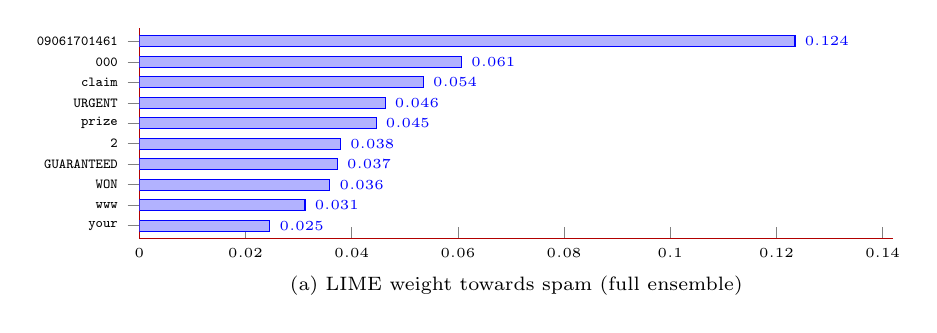
\begin{tikzpicture}
\begin{axis}[
  xbar, width=0.92\columnwidth, height=4.25cm, bar width=4.0pt,
  xmin=0, xmax=0.142, enlarge y limits=0.07,
  symbolic y coords={your,www,WON,GUARANTEED,2,prize,URGENT,claim,000,09061701461},
  ytick=data, yticklabel style={font=\tiny\ttfamily},
  xticklabel style={font=\tiny, /pgf/number format/fixed, /pgf/number format/precision=2},
  xlabel={(a) LIME weight towards spam (full ensemble)}, xlabel style={font=\scriptsize},
  nodes near coords, nodes near coords style={font=\tiny, /pgf/number format/fixed, /pgf/number format/precision=3},
  fill=red!55, draw=red!70!black, axis x line*=bottom, axis y line*=left,
]
\addplot coordinates {(0.0246,your) (0.0312,www) (0.0359,WON) (0.0373,GUARANTEED) (0.0379,2)
  (0.0446,prize) (0.0463,URGENT) (0.0535,claim) (0.0607,000) (0.1235,09061701461)};
\end{axis}
\end{tikzpicture}\\[2pt]
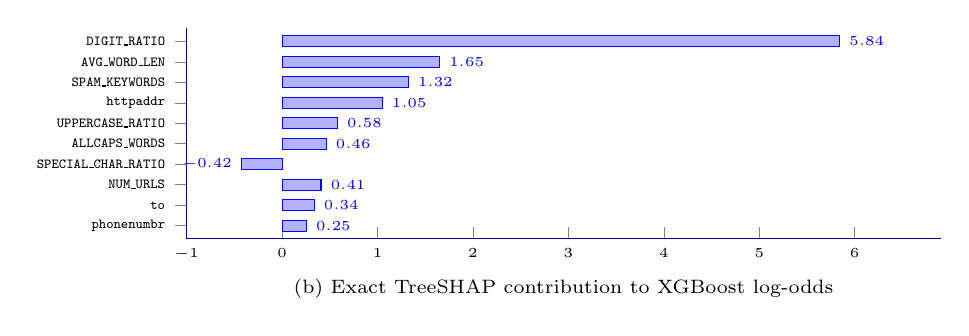
\begin{tikzpicture}
\begin{axis}[
  xbar, width=0.92\columnwidth, height=4.25cm, bar width=4.0pt,
  xmin=-1.0, xmax=6.9, enlarge y limits=0.07,
  symbolic y coords={f0,f1,f2,f3,f4,f5,f6,f7,f8,f9}, yticklabels={phonenumbr,to,NUM\_URLS,SPECIAL\_CHAR\_RATIO,ALLCAPS\_WORDS,UPPERCASE\_RATIO,httpaddr,SPAM\_KEYWORDS,AVG\_WORD\_LEN,DIGIT\_RATIO},
  ytick=data, yticklabel style={font=\tiny\ttfamily},
  xticklabel style={font=\tiny, /pgf/number format/fixed, /pgf/number format/precision=1},
  xlabel={(b) Exact TreeSHAP contribution to XGBoost log-odds}, xlabel style={font=\scriptsize},
  nodes near coords, nodes near coords style={font=\tiny, /pgf/number format/fixed, /pgf/number format/precision=2},
  fill=blue!45, draw=blue!60!black, axis x line*=bottom, axis y line*=left,
]
\addplot coordinates {(0.253,f0) (0.336,f1) (0.408,f2) (-0.424,f3) (0.461,f4) (0.580,f5) (1.049,f6) (1.322,f7) (1.650,f8) (5.842,f9)};
\end{axis}
\end{tikzpicture}
\caption{Local explanations of the illustrative smishing SMS (ensemble spam
probability 0.996): (a) LIME weights over the full ensemble; (b) the ten
largest exact TreeSHAP contributions of the XGBoost component (base value
0.50 log-odds). Upper-case names are stylometric features.}
\label{fig:local}
\end{figure}

\subsection{Global Explanations: Stylometry Rivals Vocabulary}

Fig.~\ref{fig:global} ranks features by mean absolute attribution over 800
held-out messages per channel. On SMS, eight of the ten most important
features are stylometric, led by \tok{DIGIT_RATIO}, \tok{AVG_WORD_LEN} and
\tok{SPAM_KEYWORDS}; the fifteen engineered features (0.5\% of the
dimensions) carry 74.5\% of the total attribution mass. A short scam is
betrayed by its \emph{shape}---digits, long words, capitals and
punctuation---as much as by its vocabulary. On e-mail the ranking is
dominated by a single word, \tok{enron}, whose mean attribution is about
three times that of the next feature; stylometric features
(\tok{NUM_EXCLAMATIONS}, \tok{CHAR_COUNT}, \tok{DIGIT_RATIO}) and
correspondence vocabulary (\emph{thanks}, \emph{attached}) follow.

\begin{figure}[!t]
\centering
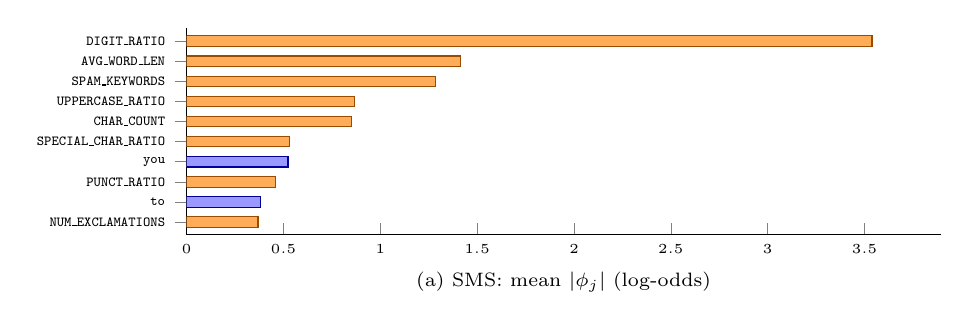
\begin{tikzpicture}
\begin{axis}[
  xbar, width=0.92\columnwidth, height=4.2cm, bar width=3.8pt,
  xmin=0, enlarge y limits=0.07,
  symbolic y coords={g0,g1,g2,g3,g4,g5,g6,g7,g8,g9}, yticklabels={NUM\_EXCLAMATIONS,to,PUNCT\_RATIO,you,SPECIAL\_CHAR\_RATIO,CHAR\_COUNT,UPPERCASE\_RATIO,SPAM\_KEYWORDS,AVG\_WORD\_LEN,DIGIT\_RATIO}, bar shift=0pt,
  ytick={g0,g1,g2,g3,g4,g5,g6,g7,g8,g9}, yticklabel style={font=\tiny\ttfamily},
  xticklabel style={font=\tiny}, xlabel={(a) SMS: mean $|\phi_j|$ (log-odds)}, xlabel style={font=\scriptsize},
  axis x line*=bottom, axis y line*=left,
]
\addplot[fill=orange!65, draw=orange!60!black] coordinates {(0.368,g0) (0.457,g2) (0.532,g4) (0.851,g5) (0.867,g6) (1.285,g7) (1.414,g8) (3.539,g9)};
\addplot[fill=blue!40, draw=blue!60!black] coordinates {(0.379,g1) (0.523,g3)};
\end{axis}
\end{tikzpicture}\\[2pt]
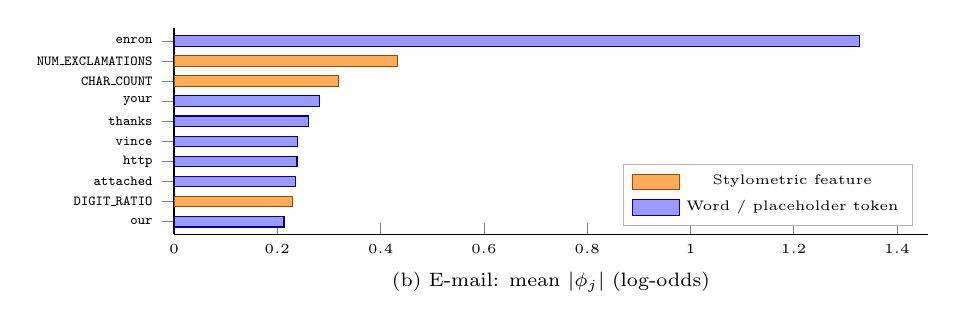
\begin{tikzpicture}
\begin{axis}[
  xbar, width=0.92\columnwidth, height=4.2cm, bar width=3.8pt,
  xmin=0, enlarge y limits=0.07,
  symbolic y coords={g0,g1,g2,g3,g4,g5,g6,g7,g8,g9}, yticklabels={our,DIGIT\_RATIO,attached,http,vince,thanks,your,CHAR\_COUNT,NUM\_EXCLAMATIONS,enron}, bar shift=0pt,
  ytick={g0,g1,g2,g3,g4,g5,g6,g7,g8,g9}, yticklabel style={font=\tiny\ttfamily},
  xticklabel style={font=\tiny}, xlabel={(b) E-mail: mean $|\phi_j|$ (log-odds)}, xlabel style={font=\scriptsize},
  axis x line*=bottom, axis y line*=left,
  area legend, legend style={font=\tiny, at={(0.98,0.04)}, anchor=south east, draw=black!30},
]
\addplot[fill=orange!65, draw=orange!60!black] coordinates {(0.229,g1) (0.318,g7) (0.432,g8)};
\addplot[fill=blue!40, draw=blue!60!black] coordinates {(0.213,g0) (0.236,g2) (0.238,g3) (0.239,g4) (0.260,g5) (0.281,g6) (1.327,g9)};
\legend{Stylometric feature, Word / placeholder token}
\end{axis}
\end{tikzpicture}
\caption{Global importance (exact TreeSHAP, XGBoost component, 800 held-out
messages per channel): the ten most important features for (a) SMS and (b)
e-mail.}
\label{fig:global}
\end{figure}

\subsection{Faithfulness of the Local Explanations}

Table~\ref{tab:lime} reports the deletion test. Removing the single
highest-ranked LIME word lowers the ensemble's spam probability by 0.106 on
average for SMS, 8.6 times more than removing a random word, and removing the
top five words lowers it by 0.455 and flips 52\% of the verdicts. For e-mail
the drops are smaller in absolute terms---long messages contain redundant
evidence---but about 20 times larger than for random deletions. LIME's
rankings therefore identify words on which the ensemble's decision genuinely
depends.

\begin{table}[!t]
\caption{Deletion Test of LIME Faithfulness: Mean Drop in Ensemble Spam Probability After Removing the Top-$k$ LIME Words / $k$ Random Words}
\label{tab:lime}
\centering
\footnotesize
\setlength{\tabcolsep}{2.4pt}
\begin{tabular}{@{}lcccc@{}}
\toprule
\textbf{Channel} & $k=1$ & $k=3$ & $k=5$ & \textbf{Flips} ($k{=}5$) \\
\midrule
\inputtable{tables/lime.tex}
\bottomrule
\end{tabular}
\end{table}

\subsection{Explanations as an Audit Tool: A Corpus Shortcut}

The prominence of \tok{enron} prompted an audit. The token occurs in 44.4\%
of legitimate training e-mails and 42.1\% of legitimate test e-mails, but in
\emph{none} of the spam messages in either split: every legitimate e-mail in
the corpus is internal Enron correspondence, so the company name is a perfect
one-sided proxy for the ham class. The attributions confirm that the model
relies on it: its mean TreeSHAP contribution is $-3.95$ log-odds (towards ham)
when the token is present, versus $+0.66$ when it is absent.
Other identity cues of the same organisation---for example the first name
\emph{vince}---also rank among the most important features. Notably,
\emph{none} of the ensemble's 35 false positives contains \tok{enron}: the
legitimate e-mails that are misclassified are precisely those lacking the
corpus marker.

Table~\ref{tab:shortcut} quantifies the consequences. Deleting the token from
523 legitimate test e-mails raises the ensemble's spam probability only
slightly (11 verdicts flip), because legitimate correspondence contains other
ham evidence. The insertion direction, however, exposes a practical evasion:
appending the single word ``enron'' to spam e-mails flips 409 of the 1,151
detected spam messages (35.5\%) to ham. Vulnerability differs sharply between
learners---XGBoost is evaded on 91.7\% of messages, RF on 25.3\% and LR on only
4.5\%---so the heterogeneous ensemble is substantially more robust than its
boosted member, yet far from immune. This shortcut is invisible in
Tables~\ref{tab:results}--\ref{tab:significance}, where the e-mail model
appears near-perfect; it became visible only through the global
explanations.

\begin{table}[!t]
\caption{Shortcut Probe on the E-mail Test Set: Inserting ``enron'' Into Detected Spam and Deleting It From Legitimate Mail}
\label{tab:shortcut}
\centering
\footnotesize
\setlength{\tabcolsep}{3.2pt}
\begin{tabular}{@{}lcccc@{}}
\toprule
 & \multicolumn{2}{c}{\textbf{Insertion into spam}} & \multicolumn{2}{c}{\textbf{Deletion from ham}} \\
\cmidrule(lr){2-3}\cmidrule(l){4-5}
\textbf{Model} & \textbf{Flips to ham} & $\overline{\Delta p}$ & \textbf{Flips} & $\overline{\Delta p}$ \\
\midrule
\inputtable{tables/shortcut.tex}
\bottomrule
\end{tabular}
\end{table}

\subsection{Computational Cost}

Table~\ref{tab:cost} summarises the cost. Training both specialists,
including 5-fold cross-validation of all three learners, takes about
1.5 minutes on a CPU. A single verdict takes about 15\,ms, an exact TreeSHAP attribution
under a millisecond, and a LIME explanation with 1,000 perturbations
0.07--0.21\,s, so every prediction can be explained interactively. Batched
scoring processes thousands of messages per second. Such task-specific models
avoid the energy cost associated with large general-purpose generative
models~\cite{luccioni2024power}.

\begin{table}[!t]
\caption{Computational Cost on a 10-Core ARM64 CPU (No GPU)}
\label{tab:cost}
\centering
\footnotesize
\setlength{\tabcolsep}{3.0pt}
\begin{tabular}{@{}lccccc@{}}
\toprule
 & \textbf{Train} & \textbf{Verdict} & \textbf{Batch} & \textbf{SHAP} & \textbf{LIME} \\
\textbf{Channel} & (s) & (ms) & (msg/s) & (ms) & (ms) \\
\midrule
\inputtable{tables/cost.tex}
\bottomrule
\end{tabular}
\end{table}

%==============================================================================
\section{Discussion}\label{sec:discussion}
%==============================================================================

\emph{Accuracy is not the bottleneck.} On both corpora all learners exceed
97\% accuracy and 0.99 ROC-AUC, and the paired tests show that a regularised
linear model on well-designed features is as accurate as the ensemble. This
agrees with recent findings that feature representation matters as much as
model complexity for short-text spam~\cite{sahin2026revisiting} and that
classical models remain competitive with transformers on phishing
e-mail~\cite{melendez2024comparative}. The ensemble's value lies in improved
ranking metrics, a better precision profile on SMS, significantly better
performance than either tree model on e-mail and---most clearly---robustness
to the shortcut attack, which the boosted model alone does not have.

\emph{Explanations change what the engineer can see.} The \tok{enron}
shortcut is a property of the corpus, not a defect of the pipeline, but a
black-box deployment would have shipped it silently, and an attacker who
learned of it could evade one third of detections with a single word. This
echoes concerns about shortcut learning in
NLP~\cite{du2024shortcut,dogra2024shortcut} and supports treating global
explanations as an auditing instrument. Explanations must themselves be
validated: the sparse/dense pitfall described in Section~\ref{sec:method}
produces plausible-looking SHAP plots of a function the deployed model does
not compute, illustrating why faithfulness has to be
tested~\cite{nauta2023anecdotal,lyu2024faithful} rather than assumed.

\emph{Practical guidance.} We recommend (i) computing tree attributions on the
exact input representation the model scores; (ii) validating local
explanations with deletion tests; (iii) inspecting global attributions for
organisation names, dates and other corpus identifiers before deployment; and
(iv) evaluating the routing step, not only the classifiers, in
multi-channel systems.

\emph{Limitations.} Both corpora are English and date from 2000--2012;
modern smishing, multilingual and code-mixed messages, and LLM-generated
phishing~\cite{heiding2024devising,opara2025evaluating} are not represented,
and the Enron-Spam shortcut means e-mail accuracy overstates performance on
other organisations' mail. Results come from a single stratified split
(complemented by cross-validation on the training data), the router is a
hand-written heuristic, SHAP explains only the boosted component, and the
faithfulness test uses a moderate number of messages. We did not benchmark a
fine-tuned transformer or an LLM under the same protocol, and adversarial
robustness beyond the shortcut probe~\cite{salman2024evasive,salman2026johnny}
was not evaluated.

%==============================================================================
\section{Conclusion and Future Work}\label{sec:conclusion}
%==============================================================================

We presented an interpretable multi-modal framework that detects scam SMS and
e-mail messages with channel-specific ensembles of Logistic Regression,
Random Forest and XGBoost and explains every verdict with LIME and exact
TreeSHAP. The ensemble reaches 98.55\% accuracy on SMS and 98.25\% on e-mail,
significantly outperforms both tree learners on e-mail, and trains in minutes
on a CPU. A deletion test confirms that its local explanations are faithful,
and its global explanations show that stylometry rivals vocabulary on SMS and
expose a corpus shortcut that a one-word insertion can exploit---an insight no
accuracy table revealed. Future work will (i) evaluate cross-corpus
generalisation and remove identity shortcuts by masking or counterfactual
augmentation, (ii) extend the framework to multilingual and code-mixed
corpora, including Indian languages, (iii) replace the heuristic router with
a learned channel classifier, (iv) add probability calibration and
counterfactual explanations, (v) benchmark transformer and LLM detectors under
the same statistical and explanation protocol, and (vi) test robustness
against obfuscation and LLM-generated scams.

\bibliographystyle{IEEEtran}
\bibliography{references}

\end{document}
